%! TEX root = ../main.tex
% ============================================================
% IMMUTABLE — generated automatically, do not edit this block
%   script          : plotter.py::plot_damping_scatter
%   plot_type       : damping_scatter
%   chapter         : 05
%   panel           : full
%   wind            : allwind
%   amplitude       : None
%   frequency       : (1.0, 1.6)
%   probes          : None
%   draft           : False
%
% DATASETS:
%   PROCESSED-20260326-ProbePos4_31_FPV_2-tett6roof-under9Mooring-height100-lowrange
%   PROCESSED-20260327-ProbePos4_31_FPV_2-tett6roof-under9Mooring30-height100-lowrange
%
% SUBFIGURES AVAILABLE:
%   FIGURES/ch05_damping_scatter_full.pdf
% ============================================================
\begin{figure}[htbp]
  \centering
  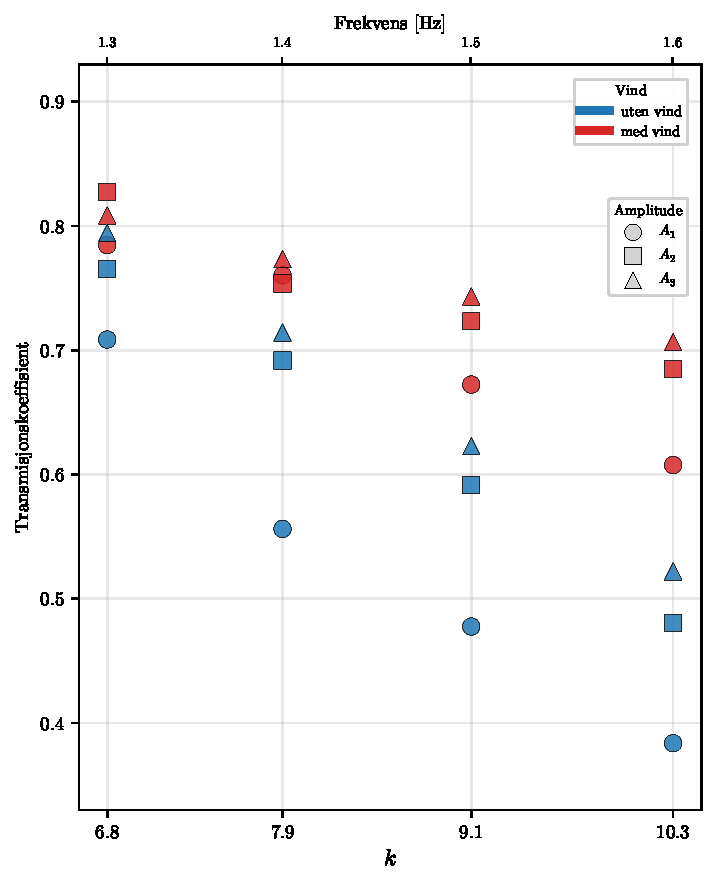
\includegraphics[width=0.9\linewidth]{FIGURES/ch05_damping_scatter_full.pdf}
  \caption[OUT/IN damping ratio versus wave frequency, all amplitudes combined]{
    OUT/IN damping ratio versus wave frequency, all amplitudes combined. full panel condition(s); colour = wind condition (full, no); marker size = wave amplitude (0.10\,V, 0.20\,V, 0.30\,V). Errorbars: standard deviation across runs.
  }
  \label{fig:ch05_damping_scatter}
\end{figure}
